\section{States}
%This section will explain the internal architecture of the launcher, this is every dependency inside the launcher.
Being able to launch an \girafapp[] as a specific guardian requires the user to interact such that the launcher knows which guardian the user represents.

Authentication was chosen, as each modulated child and guardian contains private data and therefore needs to be protected. QR-codes was chosen as means of authentication, as they provide a level of security.
An alternative to QR-codes could be a \emph{username-password} method, where each user have their own username, with an private password.
%The system is designed to have the two modes: guardian- and child mode\todo{ref to backlog}.
As explained in \autoref{backlog_childmode}\todo{tilfoej childmode til backlog}, 

The launcher is developed towards being a tool usable by both guardians and children e.g. the ``child mode'' feature, described in \autoref{backlog_childmode}\todo{tilfoej childmode til backlog}.

A username-password combination requires the user to remember their credentials, whereas some \autists[] have problems with it.

\myQuote{Some \autists[] can have problems remembering a username and password  -  Drazenko Banjak, educator at Egebakken.} \todo{Compare style to commen-rapport qoute}

QR-codes provides a physical way of storing the user credentials and allows for other users to take responsibility of the QR-code, such as a \guardian[] carrying a QR-code of a \autist[].

QR-codes can be scanned by a built-in camera on tablets and can be printed using standard paper and printer equipment. 

QR-codes are copyable, by e.g. a copymachine, and therefore must be kept away from untrusted users, if they should not be used by people for which they were not intended.

To sum up, QR-codes are chosen because of they improve usability, despite of their ability to be copied.  \\\todo{Ulrik, er dette i orden?}



\begin{figure}[h]
	\centering
	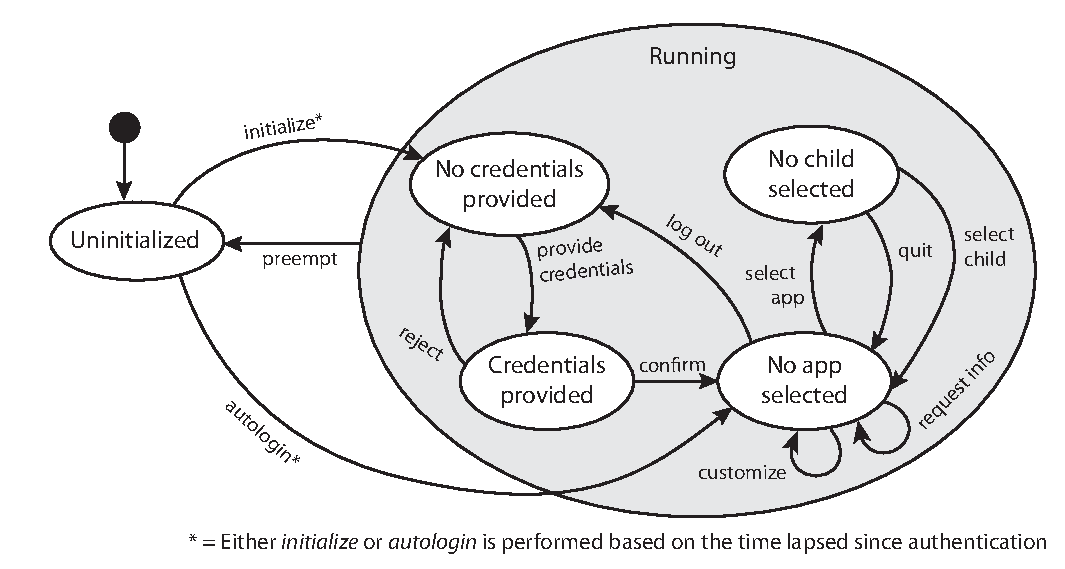
\includegraphics[width=1\textwidth]{gfx/statediagram.pdf}
	\caption{State diagram}
	\label{fig:state_diagram}
\end{figure}

\autoref{fig:state_diagram} shows all possible states and transitions, which the launcher can be in.
The ``no crendentials provided''-state is the initial state which the system is in, after initial execution.
This state, together with the ``credentials provided''-state, handles authentication and confirmation of the guardian currently using the launcher.
After confirmation, the launcher enters the ``no app selected''-state, where the launcher waits for user input, on which app to select for execution. \\

The ``no child selected''-state shows the state which the launcher is in, while waiting for user input on which child profile to use, when executing the previously selected app.
Note that the actual runtime of the selected app is not modelled here, as the launcher regardless of the selected app, transits back to the ``no app selected''-state. \\

Should the launcher be preempted by an external force, such as the OS or hardware failiure, then the launcher will enter the ``terminated''-state.
Depending on how long after authentication that the launcher is resumed after preemption, the launcher may transit to the ``no app selected''-state, instead of the ``No credentials provided''-state.
This is to take the \emph{autologin} feature -- described in \autoref{autologin} -- into account.
